\chapter{Resume (en Francais)}
\label{chapter:resume}
\pagestyle{mainmatter}
\pagenumbering{arabic}

\clearpage
\section{Brain Imaging Data Structure (BIDS)}

\begin{figure}[htb!]
\begin{center}
   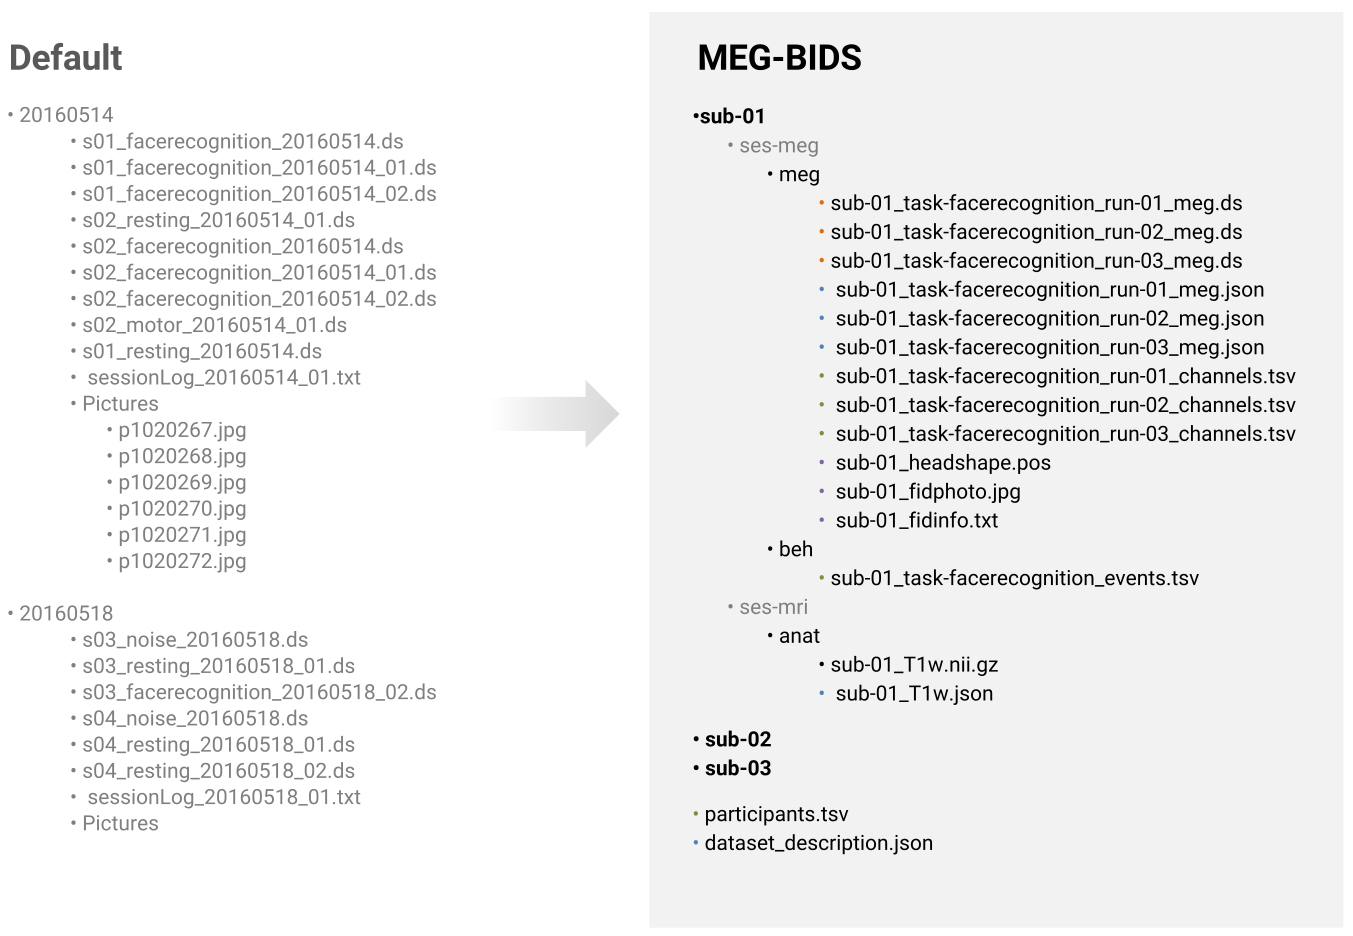
\includegraphics[width=\linewidth]{figures/bids_organization.png}
\end{center}
   \caption[BIDS-MEG data organization scheme.]{BIDS-MEG data organization scheme: Left: a typical default data organization scheme where folders are organized by date of session and contain different runs for a given participant in a study. Right: BIDS-MEG organizes data per study, then participant (subject), followed by modality, then sessions and eventually, runs. Note the sidecar files that are present at all levels of the data hierarchy, and document conveniently the metadata contents.}
   \label{fig:BIDS-MEG-organization}
\end{figure}
From the perspective of reproducibility, data sharing is of paramount importance. Sharing code by itself does not enable reproducibility if the accompanying data is not available, and expensive to acquire. Reanalysis of a dataset is however useful not just from the perspective of reproducibility but also for discovering new effects that were previously overlooked. At the same time, the more data is shared, the larger our sample sizes will be and this will enable us to conduct studies with higher statistical power. Low statistical power, as we discussed in Chapter~\ref{chapter:intro} is one of the main reasons for the reproducibility crisis.

While data sharing in neuroscience is on the rise, the amount of data reuse is still limited. For example, since the release of the Human Connectome Project (HCP)~\citep{larson2013adding} MEG data in 2013, there have been very few instances of reusing this data. At the time of writing this thesis, we had only one or two documented cases~\citep{jas2017autoreject} of reusing the HCP data. Even in these cases, the effort has mostly been limited to reproducing results rather than testing new hypotheses. This clearly represents a gap between the ideal and the practice of data sharing. 

% Clearly, sharing data is not a panacea as the tools, skills and resources to process such large datasets is currently missing in typical laboratories. Perhaps the most important roadblock is standardization of metadata.

Neuroimaging experiments are often complicated involving different  cognitive tasks (auditory, visual, somatosensory \emph{etc.}), different acquisition parameters (sampling frequency, number of sensors and their location, measurement device \emph{etc.}), and population parameters (subject's gender, age \emph{etc.}). All of this metadata is necessary information to successfully reanalyze the data. Unfortunately, historically there has been a lack of consensus amongst different labs and industrial manufacturers as to what constitutes useful metadata. This points to the need for establishing standards. While on a first glance, this may appear to be unnecessary bureaucratic red tape, in fact standards exist in almost all facets of our life. 

Apart from the meta information that is stored with the data, the data itself is stored amongst one of 10--20 different file formats and at different stages of processing. While there have been some efforts previously to standardize data structures~\citep{gibson2009minimum, grewe2011bottom, stoewer2013singlefile, teeters2015neurodata, bigdely2016preparing}, it has not gained wide acceptability. Designing a new standard is tricky as it requires gaining a community consensus. At the same time it must strike the right balance between rigidity for efficiency and flexibility for adapting to future technologies. 

The \ac{BIDS} format~\citep{gorgolewski2016brain} is indeed designed with these considerations in mind. 
The standard involves a hierarchy of folders to describe the imaging technology used, the name of the subject, and the date of the experiment. 
At each level of hierarchy, files are accompanied by sidecar \code{json} files describing the metadata. 
A \code{json} file is an easy to parse text file that contains key and value pairs, so that it has the advantage of being machine and human readable at the same time. 
These files follow an \emph{inheritance principle}, that is, a field described in a \code{json} file in a higher level of the hierarchy will be automatically propagated downstream. 
The main BIDS specification is accompanied by extension specifications which describe specific aspects to describe different modalities.
At the same time, the standard does not exist in isolation.
The \ac{BIDS} consortium is also providing a growing ecosystem of tools to convert datasets into \ac{BIDS} compatible format as well as to validate data to conform to the standard. 

In the present work, we present a significant extension of \ac{BIDS} to support the specific aspects of \ac{MEG} data. \Ac{MEG}, as we know from Chapter~\ref{chapter:intro}, provides direct measurement of brain activity with millisecond temporal resolution and unique source imaging capabilities. So far, \ac{BIDS} has provided a solution to structure the organization of \ac{MRI} data. Despite the lack of standard data format for \ac{MEG}, BIDS-MEG is a principled solution to store, organize and share the typically-large data volumes produced. It builds on \ac{BIDS} for \ac{MRI}, and therefore readily yields a multimodal data organization by construction. This is particularly valuable for the anatomical and functional registration of \ac{MEG} source imaging with \ac{MRI}. With BIDS-MEG and a growing range of software adopting the standard, the \ac{MEG} community has a solution to minimize curation overheads, reduce data handling errors and optimize usage of computational resources for data analysis. The standard also includes well-defined metadata to facilitate future data harmonization and sharing efforts, and extensions to other electrophysiological data modalities.

\clearpage
\section{A reproducible M/EEG group study}

\begin{figure}[t]
  \centering
  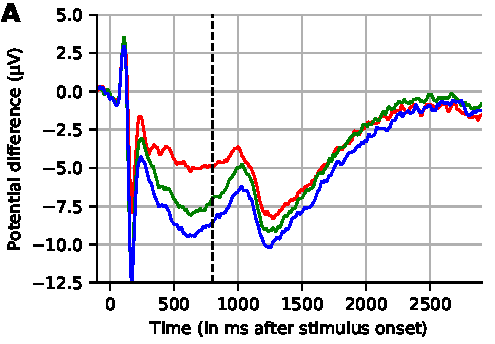
\includegraphics[width=0.7\linewidth]{figures/grand_average_highpass-NoneHz.pdf}\\
  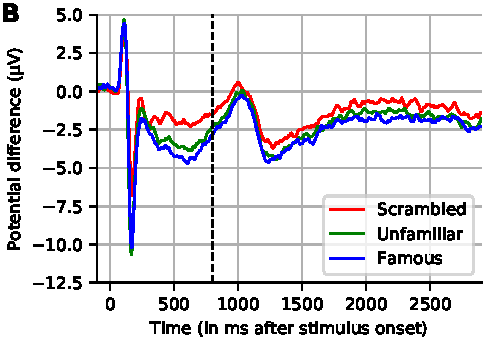
\includegraphics[width=0.7\linewidth]{figures/grand_average_highpass-1Hz.pdf}
\caption[Grand averaged evoked response across 16 subjects.]{Grand averaged evoked response across 16 subjects for channel EEG065.
(A) No highpass filter. (B) Highpass filtered at 1.0 Hz. Note that, similar to (A), the results reported by \cite{wakeman2015multi} (dashed line at 800 ms indicates where their plot stopped) show large drifts, but these return to near-baseline levels toward the end of a sufficiently long interval (here, 2.9 seconds) even without applying a highpass filter.}
\label{fig:grand_average}
\end{figure}  

In the previous chapter, we discussed how data sharing can be facilitated using the \ac{BIDS} for \ac{MEG}. This is taking us one step closer to the goal of reproducibility. However, reproducibility is not achieved by merely sharing more data with the hope that this will solve all problems. As noted in \citet{baker20161}, one of the best solutions to foster reproducible science is not a technical one, but an educational one. This is of course true for statistics, where there is an urgent need to clarify and educate researchers about the statistical tools required in neuroscience. But it is now increasingly important also for academic software.

In recent years, free academic toolboxes have gained increasing prominence in \ac{MEG} analysis as a means to disseminate cutting edge methods, share best practices between different research groups and pool resources for developing essential tools for the \ac{MEG} community. Teaching events are regularly held around the world where the basics of each toolbox are explained by its  developers and experienced power users. There are however, knowledge gaps that need to be addressed. First, most teaching examples only show analysis of a single ‘typical best’ subject whereas most real MEG studies involve analysis of group data. It is then left to the researchers in the field to figure out for themselves how to make the transition and obtain significant group results. Secondly, we are not familiar with any examples of fully analyzing the same group dataset with different academic toolboxes to assess the degree of agreement in scientific conclusions and compare strengths and weaknesses of various analysis methods and their independent implementations.

To address this very issue, a workshop was organised by the lead developers of six most popular free academic MEG toolboxes at Biomag 2017. This work is a follow up to the workshop, which presents the contribution of the MNE software team, and will be published in \emph{Frontiers in Neuroscience, section Brain Imaging Methods}. This study presents the results obtained by the reanalysis of an open dataset from \citet{wakeman2015multi} using the MNE software package. The analysis covers preprocessing steps, quality assurance, sensor-space analysis of evoked responses, source localization, and statistics in both sensor and source space. Results with possible alternative strategies are presented and discussed at different stages such as the use of high-pass filtering versus baseline correction, tSSS versus \ac{SSS}, the use of a minimum norm inverse versus \ac{LCMV} beamformer, and the use of univariate or multivariate statistics. This aims to provide a comparative study of different stages of \ac{MEG}/\ac{EEG} analysis pipeline on the same dataset, with open access to all of the scripts necessary to reproduce this analysis.

\clearpage

\section{Automated artifact rejection for M/EEG}

\begin{figure}[t]
	\centering
	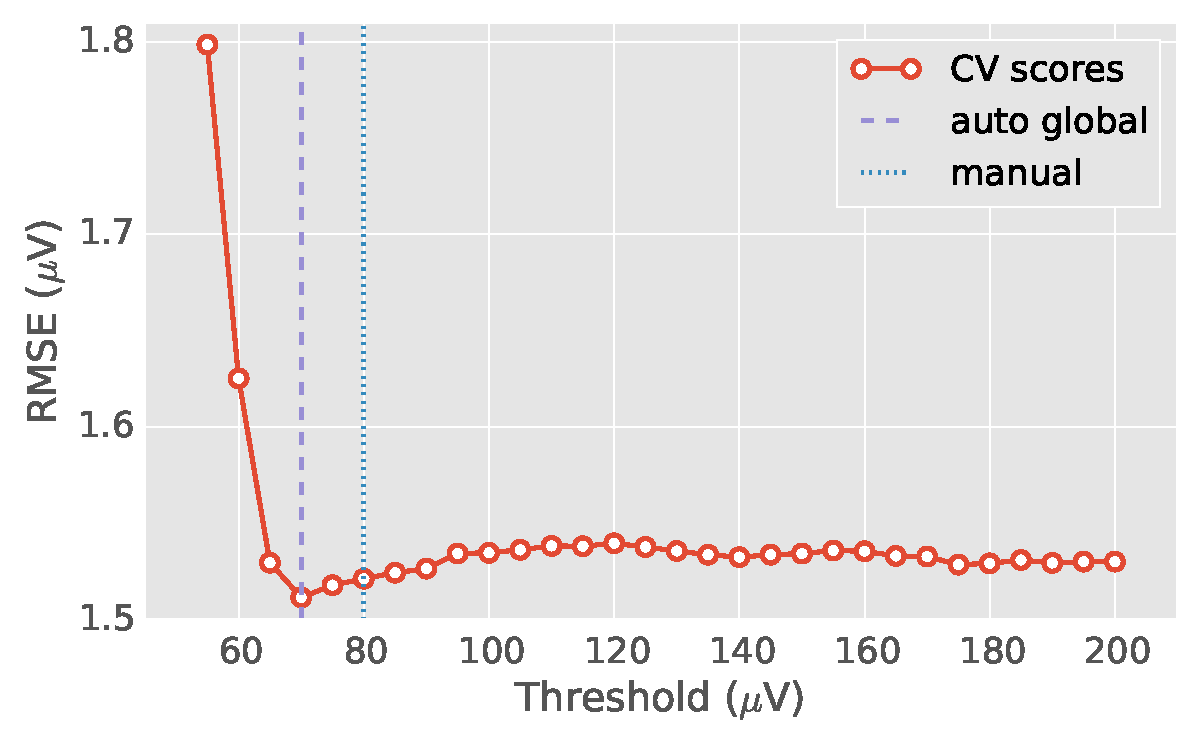
\includegraphics[width=0.8\linewidth]{figures/figure1.pdf}
    \caption[Cross-validation error as a function of peak-to-peak rejection threshold on one EEG dataset.]{Cross-validation error as a function of peak-to-peak rejection threshold on one EEG dataset. The root mean squared error (RMSE) between the mean of the training set (after removing the trials marked as bad) and the median of the validation set was used as the cross-validation metric (Section~\ref{sec:auto_global}). The two insets show the average of the trials as ``butterfly plots" (each curve representing one sensor) for very low and high thresholds. For low thresholds, the RMSE is high because most of the trials are rejected (underfit). At high thresholds, the model does not drop any trials (overfit). The optimal data-driven threshold (\emph{autoreject, global}) with minimum RMSE is somewhere in between. It closely matches the human threshold.}
    \label{fig:cross_val}
\end{figure}

In the last chapter, we discussed the reproducibility challenges when performing group studies in \ac{MEG} and \ac{EEG}. One way to improve reproducibility is automation, and we briefly touched upon an algorithm for automating detection of bad data segments, known as \emph{autoreject}.

%copy pasted abstract below
In this chapter, we will present this algorithm which rejects and repairs bad trials in \ac{MEG} and \ac{EEG} signals. Annotating bad segments in the data is perhaps one of the most time consuming aspects of data processing in electrophysiology. Currently, it is either done manually, or using automated black-box algorithms. The manual approach is often subjective with often no clear consensus on what constitutes a corrupted data segment. Therefore, reanalysis is not only manually demanding but can also lead to problems in reproducibility. On the other hand, the automated methods are controlled by parameters that are not straightforward to tune. In the case of failure, it is not always obvious what caused the method to fail and how it can be corrected. As a result, one is left with no choice but to exclude the data from further analysis.

This led us to develop a method based on design choices motivated by ease of interpretation and diagnosis. The method we propose capitalizes on cross-validation in conjunction with a robust evaluation metric to estimate the optimal peak-to-peak threshold--a quantity commonly used for identifying bad trials in \ac{MEG}/\ac{EEG}. This approach is then extended to a more sophisticated algorithm which estimates this threshold for each sensor yielding trial-wise bad sensors. Depending on the number of bad sensors, the trial is then repaired by interpolation or by excluding it from subsequent analysis. For efficiency reasons, we use Bayesian optimization which is a well-known technique for hyperparameter optimization. All steps of the algorithm are fully automated thus lending itself to the name \emph{autoreject}. Crucially, the algorithm is even able to deal with sensors that are locally corrupted, which is quite often the case for \ac{EEG} data.

In order to assess the practical significance of the algorithm, we conducted extensive validation and comparisons with state-of-the-art methods on four public datasets containing \ac{MEG} and \ac{EEG} recordings from more than 200 subjects. The comparisons include purely qualitative efforts as well as quantitatively benchmarking against human supervised and semi-automated preprocessing pipelines. The algorithm allowed us to automate the preprocessing of \ac{MEG} data from the \ac{HCP} going up to the computation of the evoked responses. The automated nature of our method minimizes the burden of human inspection, hence supporting scalability and reliability demanded by data analysis in modern neuroscience.

\clearpage
\section{Temporal representation learning}

So far, we studied automation in neuroimaging with the objective of enabling scalable data analysis and reproducibility. While  reproducibility and large-scale data analysis allow us to consolidate upon existing studies, \emph{per se} they are not tools to uncover new and interesting phenomena. In this chapter, we will explore this dimension of automation using what is known as \emph{representation learning}.

Representations are the building blocks of signal processing. It is quite easy to convince ourselves of this fact, if we simply use a Fast Fourier Transform (FFT) to filter data. When we are using an FFT, we are in effect, decomposing the signal into a sum of sinusoids of varying frequencies. If we are interested in a time-frequency analysis, a common choice of representation for neurosience signals consists in using Morlet wavelets.

Traditionally, the choice of representation has been mainly driven by analytical concern and ease of mathematical manipulation. However, the recent surge of deep learning has ignited an interest in data-driven representations. It is because good representations  that compactly capture the properties of the data are essential for efficient and accurate learning systems. In computer vision, for instance, handcrafted features such as SIFT~\citep{lowe1999object} and GIST descriptors~\citep{oliva2001modeling}, Deformable Parts Model (DPM)~\citep{felzenszwalb2010object}, Histogram of Oriented Gradient (HOG)~\citep{dalal2005histograms} \emph{etc.} had been the norm, before it was realized that unsupervised learning and autoencoders performed much better.

Today, unsupervised learning is used as a first step for a supervised learning task in computer vision. Representation learning, by itself, is perhaps not as interesting, except for diagnostic visualizations in deep learning~\citep{zeiler2014visualizing}. Despite this, there has always been an interest in understanding representations in the human brain (visual system particularly), as it was thought that this would help us build better learning systems. One of the pioneers in this area of research is Bruno Olshausen, whose work on dictionary learning~\citep{olshausen1996emergence} demonstrated that Gabor patches are indeed fundamental to natural images, similar to the ones that Hubel and Wiesel~\citep{hubel1962receptive, marcelja1980mathematical} found in the cat visual cortex, and to what is used in GIST features. Barring this line of studies, the learned representation itself is not considered as meaningful as performance metrics like the prediction score or reconstruction loss. However, in the case of neural signals, we realized that this is not the case and the fidelity of the representation is in itself interesting. Indeed, the shape of the signal is a crucial biomarker in many clinical applications for neuroscience~\citep{cole2017brain}. 

A parallel development in the field of neuroimaging has been the rise in interest for learning prototypical shapes which are shift invariant~\citep{jost2006motif, barthelemy2013multivariate, brockmeier2016learning, hitziger2017adaptive}. It is motivated by the fact that existing approximations using the Fourier basis often distorts the signal. There is, for example, a debate regarding the type of filters that should be used (See Section~\ref{sec:group_study_temporal_filtering} and \cite{widmann2015digital,parks1987digital,ifeachor2002digital, gotz-etal:15}). 
Even though some success has been reported
with these algorithms in neuroimaging, they are limited in applicability due to their heuristic nature.
Remarkably, there has been so far very little cross-pollination of ideas between the computer vision and neuroimaging communities on these sparse coding aspects. 
Our work is an attempt to bridge this gap. 
We propose a model which builds upon existing shift-invariant sparse coding models to be able to handle heavy-tailed noise and artifacts. It assumes positivity of the coefficients to account for the fact that an atom does not change polarity over time. 

Our model is a novel probabilistic \ac{CSC} model for learning shift-invariant atoms from unprocessed neural time series data containing
potentially severe artifacts.
In the core of our model, which we call $\alpha$CSC, lies a family of heavy-tailed
distributions called $\alpha$-stable distributions. We develop a novel, computationally efficient Monte Carlo
expectation-maximization algorithm for inference. The maximization step boils down to a weighted
\ac{CSC} problem, for which we develop a computationally efficient optimization algorithm.

In our work, we rigorously evaluate the computational efficiency of our algorithm against the competing benchmarks. Because the \ac{CSC} problem is non-convex, the optimization procedure involves nested loops and theoretical analysis often falls short in dealing with the complexity of non-convex functions. 
The optimization procedure is nested as the problem is convex when one of the variables is fixed: the atoms or the activations. The outer loop alternates between these two variables while the inner loop learns them when the other is fixed. An experimental approach, while challenging, is not completely out of reach. The final result depends on the initialization, and therefore algorithms can be compared only if they are tested for many different random seeds and their results averaged. Our qualitative analysis also goes beyond the narrative of verifying the existence of known waveforms to uncovering more complex structures in the data.

Our results
show that the proposed algorithm achieves state-of-the-art convergence speeds. Besides, $\alpha$CSC is
significantly more robust to artifacts when compared to three competing algorithms: it can extract
spike bursts, oscillations, and even reveal more subtle phenomena such as cross-frequency coupling
when applied to noisy neural time series.

\begin{figure}[t]
    \centering
     \subfigure[$K=10$, $L=32$.]{
     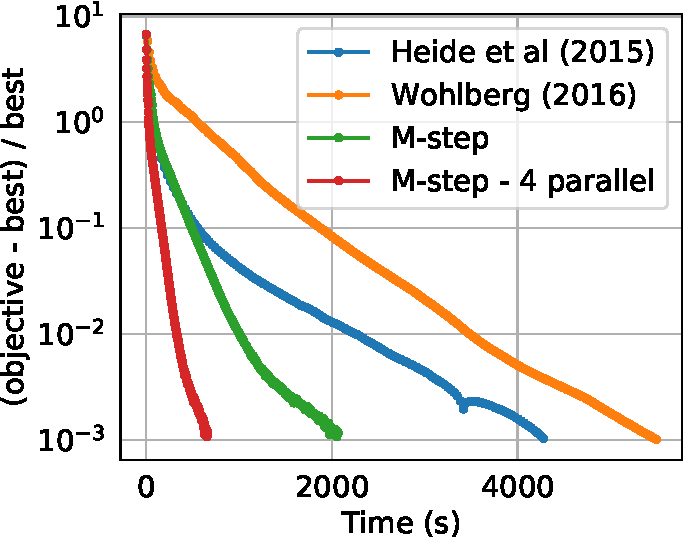
\includegraphics[width=0.5\linewidth]{figures/relative_10_32.pdf}} \\
     \subfigure[Time to reach a relative precision of 0.01.]{
     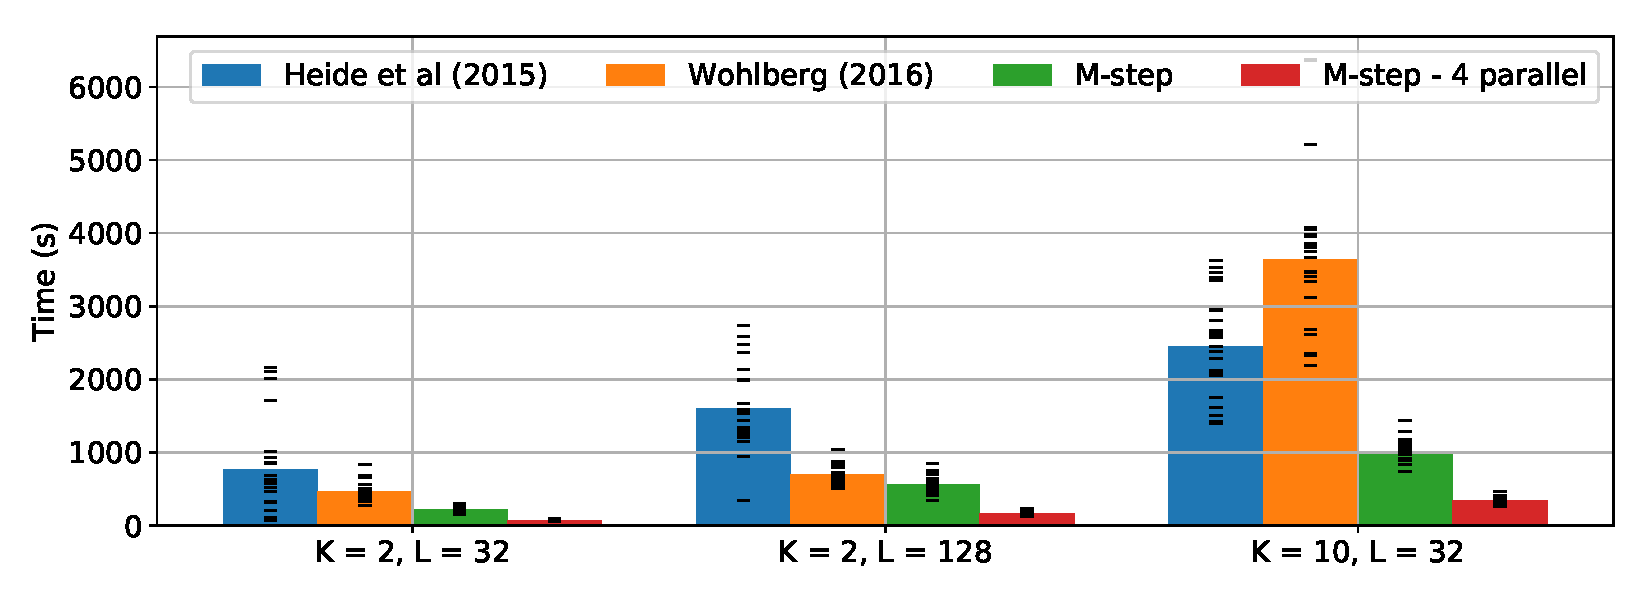
\includegraphics[width=\textwidth]{figures/bar_plot.pdf}}
    \caption[Comparison of state-of-the-art methods with our approach.]{Comparison of state-of-the-art methods with our approach. (a)~Convergence plot with the objective function relative to the obtained minimum, as a function of computational time. (b)~Time taken to reach a relative precision of $10^{-2}$, for different settings of $K$ and $L$.  }
    \label{fig:convergence}
\end{figure}

\begin{figure}[b]
    \centering
             \subfigure[LFP spike data from \cite{hitziger2017adaptive}]{
             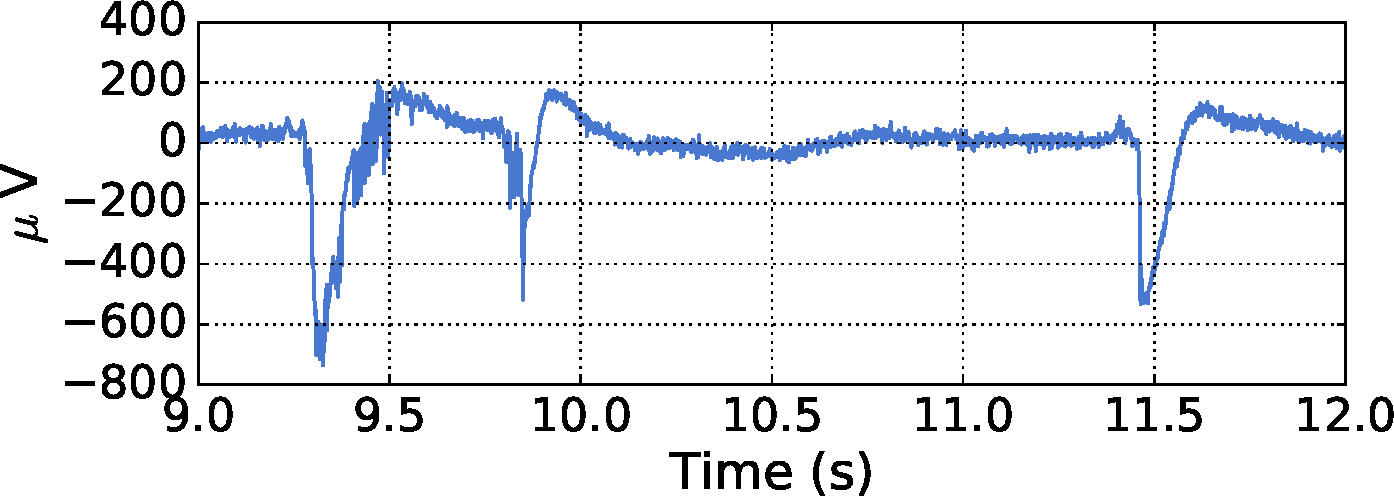
\includegraphics[height=3cm]{figures/spike_atomsa.pdf}
             \label{fig:spikedata}}
             \subfigure[Estimated atoms]{
             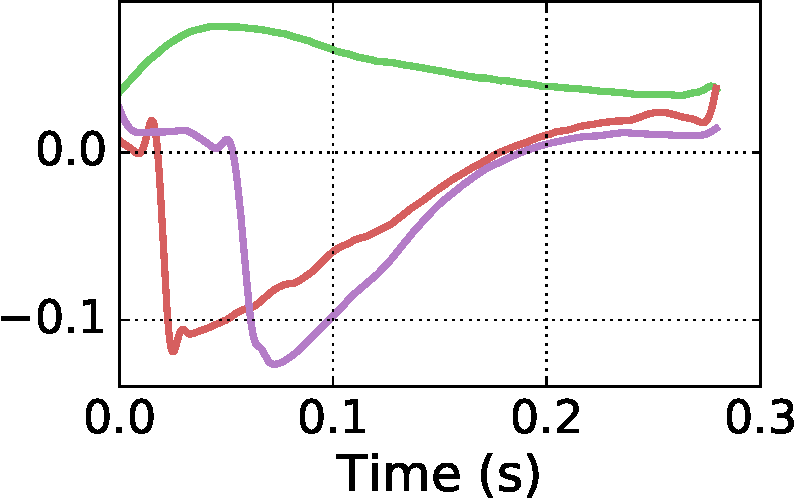
\includegraphics[height=2.9cm]{figures/spike_atomsb.pdf}
             \label{fig:spikeatoms}}

            \caption[Atoms learnt by $\alpha$CSC on LFP data containing epileptiform spikes with $\alpha=2$.]{Atoms learnt by $\alpha$CSC on LFP data containing epileptiform spikes with $\alpha=2$.}
\end{figure}
